\section{Introducción}
A lo largo de este tema vamos a estudiar la teoría de la disponibilidad de los sistemas distribuidos así como algunas arquitecturas que permiten obtener un incremento de la misma.

Para empezar debemos definir qué es la disponibilidad.

\begin{defn}[Disponibilidad]
La disponibilidad de un sistema es la probabilidad de que este se encuentre operativo en un instante de tiempo determinado.
\end{defn}

Hay dos motivos por los que un sistema puede no estar disponible:
\begin{enumerate}
\item[1] \textbf{Paradas no planificadas}

Este tipo de paradas se deben a fallos en los equipos o en los programas que implementan los servicios.

Requieren tratamiento estadístico, pues no habrá dos iguales. Los sistemas que las minimizan se llaman de \textbf{Alta Disponibilidad} \textit{(High Availability, HA)}\index{High!  Availability} \index{HA}


Algunas de las causas más frecuentes por las que se producen este tipo de paradas son:

\begin{itemize}
\item Extensión del tiempo destinado a operaciones planificadas.
\item Error humano.
\item Fallo en aplicación.
\item Fallo del sistema operativo.
\item Fallo hardware.
\item Errores de configuración del software.
\end{itemize}

\item[2] \textbf{Paradas planificadas}

Son requeridas por la aplicación para su correcto funcionamiento: Rearranques programados, copias de seguridad, cambios de configuración...

Por ser previsibles permiten un tratamiento sistemático. Los sistemas que las minimizan se denominan de \textbf{Operación Continua} \textit{(Continuous Operation, CO)} \index{Continuous! Operation} \index{CO}

Algunas de las causas más frecuentes por las que se producen este tipo de paradas son:

\begin{itemize}
\item Copias de seguridad.
\item Reemplazar o actualizar hardware.
\item Reemplazar o actualizar aplicaciones.
\item Actualizar sistema operativo.
\item Instalación de parches
\end{itemize}
\end{enumerate}

Evidentemente, un sistema ideal sería de Alta Disponibilidad y de Operación Continua. No obstante, a mayor disponibilidad del sistema mayor es el coste del mismo y su mantenimiento. Por tanto, es necesario valorar el nivel de disponibilidad requerido para un funcionamiento aceptable e invertir lo necesario para conseguirlo sin tratar de superarlo.

Antes de seguir estudiando el tema de la disponibilidad, vamos a ver una serie de definiciones de términos que aparecerán a lo largo de los apuntes y que es necesario precisar.

\begin{defn}[Fiabilidad (Reliability)][Fiabilidad]\index{Reliability}
Probabilidad de que un componente o sistema continúe funcionando en un determinado instante en el tiempo.
\end{defn}

\begin{defn}[Elasticidad o Resiliencia (Resiliency)][Resiliencia]\index{Elasticidad}\index{Resiliency}
Capacidad de un sistema para adaptarse a
condiciones externas imprevistas (fallos, aumento de carga...) para continuar cumpliendo sus parámetros de calidad.
\end{defn}

\begin{defn}[Mantenibilidad (Serviceability)][Mantenibilidad]\index{Serviceability}
Es la probabilidad de realizar una reparación satisfactoria en un tiempo determinado.
\end{defn}

\begin{defn}[Sistemas\IS tolerantes a fallos (Fault-Tolerant Systems)][Sistemas\IS tolerantes a fallos]\label{cluster:FT}
Sistemas que contienen
componentes hardware dobles de modo que el fallo de uno de ellos no suspende su
operación.
\end{defn}
\newpage
\begin{defn}[Clusters\IS de alta disponibilidad (High Availability Clusters)][Clusters\IS de alta disponibilidad]
Conjunto de nodos de servicio que comparten conexiones externas (red, discos...) y están gestionados por un software especial que permite proporcionar servicio sin interrupciones ante el fallo de alguno de sus componentes.
\end{defn}

\begin{defn}[Clusters\IS de alto rendimiento (High Performance Clusters)][Clusters\IS de alto rendimiento]\label{cluster:HP}
Conjunto de nodos de servicio que comparten una misma carga de trabajo.
\end{defn}

\begin{defn}[Recuperación ante desastres (Disaster Recovery)][Recuperación\IS ante desastres]
Capacidad de una instalación de
recuperar la operatividad tras un evento de gran magnitud, bien de tipo local (edificio), urbano (ciudad) o regional (área extendida con infraestructuras comunes).
\end{defn}

\section{Teoría de la disponibilidad}
\subsection{Disponibilidad}
La disponibilidad, $A$, de un sistema se estima a partir de la medida del tiempo que ha estado operativo, $T_{op}$, en un intervalo de tiempo, $T_{tot}$, suficientemente grande.
\[A= \frac{T_{op}}{T_{tot}}\]

Pero esta medida no da una idea global de la disponibilidad del sistema, pues un mismo valor puede obtenerse de la misma forma.

Por ejemplo, no es lo mismo que un sistema esté disponible 99 horas de cada 100 que 99 segundos de cada 100. Incluso si dos datos se han obtenido dividiendo los datos en las mismas unidades y estamos, por ejemplo, en 99 horas de cada 100 de actividad, puede ser que el sistema haya fallado una única vez en esas 99 horas y tardase una hora en recuperarse o que el sistema falle cada media hora tardando poco en recuperarse.

Por ello se utilizan otras medidas para estudiar la disponibilidad del sistema.

\begin{defn}[Tiempo medio\IS entre fallos]

En inglés \textbf{Mean Time Between Failures, MTBF}, es valor esperado del tiempo que transcurre entre dos fallos consecutivos de un equipo.
\end{defn}

\begin{defn}[Tiempo medio\IS hasta el fallo]

En inglés \textbf{Mean Time To Failure, MTTF}, es el valor esperado del tiempo de vida de un equipo o sistema, medida de su Fiabilidad (Reliability).
\end{defn}

\begin{defn}[Tiempo medio\IS de reparación/recuperación]

En inglés \textbf{Mean Time To Repair/Restore, MTTR}, es el valor esperado del tiempo que se tarda en sustituir un equipo averiado o recuperar un fallo de software.
\end{defn}

A partir de estos valores se calcula la disponibilidad según la fórmula:

\[A=\frac{MTTF}{MTBF}=\frac{MTTF}{MTTF+MTTR}\]

Para pasar de la primera a la segunda fórmula se emplea la relación lógica $MTBF=MTTF+MTTR$, es decir, el tiempo que transcurre entre dos fallos es la suma del tiempo que tarda en recuperarse el sistema tras un fallo más el tiempo que tarda en volver a fallar.

\subsection{Fiabilidad}

La fiabilidad de un componente o sistema en el tiempo es la probabilidad de que el sistema continúe funcionando en un instante de tiempo. Si denominamos $T$ al tiempo de vida del componente, su fiabilidad viene dada por la expresión:
\[R(t)=\mathbb{P}\{T > t \}\]

La vida del componente, $T$, es una variable aleatoria, cuya función de distribución es
\[F_T(t)=\mathbb{P}\{T \leq t \}\]

Evidentemente ambas variables probabilidades deben sumar siempre 1, $R(t)+F_T(t)=1$ y derivando obtenemos que sus funciones de densidad son iguales pero de signo contrario.

Una vez hemos definido estas variables podemos definir el tiempo medio hasta fallo como la esperanza de vida de un componente:
\[MTTF = E[T]=\int_{-\infty}^{\infty}fF'_T(t)dt\]

Ahora, sabiendo algo de probabilidad, podemos calcular la probabilidad de que un sistema falle antes de un instante, $x$, sabiendo que funcionaba en un instante $t<x$.
\[F_T(x | T > t ) = \mathbb{P}\{T \leq x | T> t\}=\frac{\mathbb{P}\{(T \leq x) \cap (T > t)\}}{\mathbb{P}\{T > t\}}=\frac{\mathbb{P}\{t < T \leq x\}}{\mathbb{P}\{T > t\}}=\]
\[=\frac{F_T(x)-F_T(t)}{1-F_T(t)}\]

y derivando con respecto a $x$ se obtiene
\[f_T(x | T > t)=\frac{f_T(x)}{1-F_T(x)}\]

A partir de esta última expresión se define la \concept{función de tasa de fallo} al evaluarla en $x=t$.
\[r(t)=f_T(t | T > t)=\frac{-R'(t)}{R(t)}\]

y se interpreta como la probabilidad de que un componente que funciona falle en el instante siguiente:
\[\mathbb{P}\{t<T\leq t + dt | T > t\}=f_T(t | T > t)dt=r(t)dt\]

Si la tasa de fallos tiene un valor constante, integrando la función $r(t)$ entre $0$ y $t$ y despejando $R(t)$ llegamos a:
\[R(t)=e^{-λt} \implies F_T(t) = 1-e^{-λt}\]

con lo que acabamos de obtener que el tiempo de vida es una distribución exponencial y su valor esperado será el MTTF=1/λ

\subsection{Distribución de los fallos}

La función de tasa de fallos en un equipo tiene la forma que se muestra en la figura:
\begin{center}
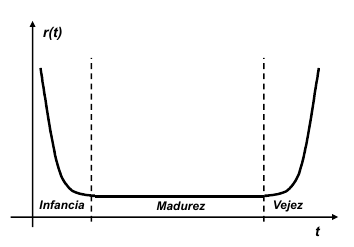
\includegraphics[width=0.7\linewidth]{img/tasa_fallos.png}
\end{center}

Durante la zona de infancia la tasa de fallos es alta debido al montaje de componentes defectuosos. Esta tasa de fallos se reduce con el tiempo hasta alcanzar una etapa de madurez que se correspondería con la época en que tenemos tasa de fallos constante. Por último el envejecimiento del equipo aumenta la tasa de fallos.

Todos los cálculos se realizan pensando en la zona de madurez del equipo, trabajando con $r(t)=cte$

Por otro lado tenemos también los fallos en programas que pueden dividirse en dos tipos según su tratamiento
\begin{enumerate}
\item[1] Programas que no son reparados cuando se encuentra el fallo sino que es necesario esperar a que se publique una nueva versión del mismo. Es la situación habitual en producción y con programas cerrados.

El modelo de tasa de fallos constante es válido durante el uso de una misma versión. Al cambiarla es necesario recalcular todos los datos.

\item[2] Programas cuyos defectos se corrigen conforme se encuentran. Suele tratarse de programas de producción propia o ciclos de pruebas en la producción de programas. El principal problema es que la solución de un defecto puede y suele introducir otros nuevos.

En este caso el modelo de tasa de fallos constante no es válido ya que tendremos una tasa de fallos que decrece con el tiempo (según se van arreglando los desperfectos). Su forma depende del modelo elegido para el ritmo de descubrimiento de fallos.

\end{enumerate}

\subsection{Mantenibilidad}
Es la probabilidad de realizar una reparación satisfactoria en un tiempo determinado. Mide la rapidez y facilidad con que un sistema se vuelve a poner operativo tras un fallo.
\[M(t)=\mathbb{P}\{T'> t\} \text{ con T' el tiempo de reparación}\]

Este tiempo incluye el tiempo necesario para descubrir el fallo, encontrar la causa, conseguir las piezas necesarias, la instalación de las mismas, arrancar el sistema de nuevo, etc. Es decir, incluye todo el tiempo gastado desde que \textbf{se produce} el fallo (aún si no se detecta) hasta que se resuelve el problema.

\[MTTR=E[T']\]

\subsection{Componentes en serie frente a Componentes en paralelo}

Si tenemos un sistema compuesto por componentes en serie, un fallo en cualquiera de ellos implica un fallo global. La conexión en serie puede no ser física pero si lógica, una componente depende del resultado del trabajo de otra.

Suponiendo que el fallo en cada componente es independiente del resto, tenemos:
\[A= \prod_{i=1}^{n}A_i; \ \ \; R(t)=\prod_{i=1}^{n}R_i(t); \  \ \; r(t)=\sum_{i=1}^{n}r_i(t)\footnote{No veo clara esta fórmula}\]

Si tenemos un sistema compuesto por componentes en paralelo y estas componentes son redundantes para su funcionamiento, un fallo en una de ellas no implicará un fallo en el sistema.

Suponiendo que el fallo en cada componente es independiente nos queda:
\[A= 1-\prod_{i=1}^{n}(1-A_i)\footnote{Estará disponible cuando al menos una componente esté disponible}; \ \ \; F_T(t)=\prod_{i=1}^{n}F_{T_i}(t); \  \ \; R(t)= 1-\prod_{i=1}^{n}(1-R_i(t))\]

\begin{center}
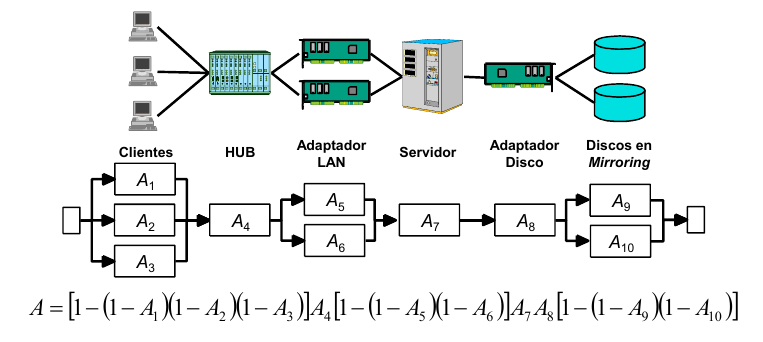
\includegraphics[width=\linewidth]{img/disponibilidad.png}
\end{center}



\section{Mejoras de la disponibilidad}

Recordemos la ecuación inicial que dimos para la disponibilidad:
\[A=\frac{MTTF}{MTTF+MTTR}=\frac{1}{1+MTTR/MTTF}\]

simplemente viendo esta fracción podemos ver que la disponibilidad de un sistema puede mejorarse (aumentar) de dos formas:
\begin{itemize}
\item Aumentando $MTTF$ mejorando la calidad de los equipos, introduciendo redundancias o eliminando \textbf{Puntos Simples de Fallo}

\item Reduciendo $MTTR$ mediante la reducción del tiempo empleado en cualquiera de las siguientes fases:
\begin{itemize}
\item Tiempo de \textbf{latencia} (desde que se da el fallo hasta que se descubre que algo falla)

\item Tiempo para aislarla (desde que se descubre hasta que se encuentra el motivo)

\item Tiempo para corregirla

\item Tiempo para verificar que todo funciona bien
\end{itemize}
\end{itemize}

\subsection{Arquitecturas que incrementan la disponibilidad}

La disponibilidad de una cadena de procesamiento es siempre menor que la menor de las disponibilidades de sus componentes. Denominamos \concept{Single Point Of Failure, SPOF} a los puntos más críticos del sistema, aquellos que al fallar implican la caída del servicio.

Como es evidente, la forma en que más podemos incrementar el $MTTF$ de cada componente es mediante la creación de un \textbf{cluster} (elementos redundantes) en cada parte de la cadena de procesamiento. Esta solución, además, elimina los SPOF al añadir redundancias incluso a esos componentes más críticos.

Conseguir que varios sistemas realicen en paralelo una misma función no es sencillo y la solución empleada depende de factores como el tipo de elemento al que se le quiere dar redundancia y las necesidades de disponibilidad del sistema completo.

En cualquier caso, siempre es necesario considerar dos procesos a la hora de implementar un sistema: el cómo actuar cuando se produce un fallo para poder mantener el servicio, \concept{Fail-over}, y cómo actuar para recuperar la situación normal una vez se resuelve el fallo \concept{Fail-back}.

Existen diferentes tipos de redundancia:
\begin{enumerate}
\item[1] \textbf{Según el estado de cada elemento del cluster}

Pueden estar todos los elementos activos (AA), uno activo y el resto preparados para activarse casi instantáneamente (AS) o uno activo y el resto detenidos pudiendo activarse en un cierto periodo de tiempo (AP)

\item[2] \textbf{Según el reparto de carga entre los elementos del cluster}

Puede ser dinámico (D), en cuyo caso no habrá que preocuparse en caso de fallo de un componente; o estático (E), donde un fallo implica reconfigurar el reparto de carga

\item[3] \textbf{Según el tratamiento de las conexiones activas}

Las sesiones activas pueden continuar (C) tras un fallo o ser interrumpidas (I).
\end{enumerate}

\section{Redundancia en los sistemas de comunicaciones}
Los sistemas de comunicaciones son uno de los puntos críticos de todo sistema distribuido.

Vamos a distinguir la redundancia en las redes de área local (LAN) y en redes de área extendida (WAN) considerando en ambos casos los estándares de facto actuales: redes LAN basadas en Ethernet y TCP/IP como medio de transporte.

Las características de los equipos que actualmente se emplean para implementar una LAN hacen que estas redes se puedan construir atendiendo a tres modelos distintos:
\begin{itemize}
\item \textbf{Nivel 2 compartido} Múltiples servidores se conectan a un mismo segmento de LAN implementado en un \textit{Hub}. Es el menos utilizado por ser el menos eficiente y flexible.

El \textit{hub} es un dispositivo que tiene la función de interconectar las computadoras de una red local. Su funcionamiento es más simple comparado con el \textit{Switch} y el \textit{router}:
El \textit{hub} recibe datos procedentes de una computadora, los transmite a los demás. En el momento en que esto ocurre, ninguna otra conmutadora puede enviar una señal. Su liberación surge después que la señal anterior haya sido completamente distribuida.


\item \textbf{Nivel 2 conmutado} Cada enlace es un segmento de LAN. Todos los componentes se interconectan mediante \textit{switches}, que actúan como puentes multipuerta.

Suele emplearse en el \textbf{nivel de acceso}, por ejemplo, en las conexiones de los ordenadores de las granjas de servidores.

\item \textbf{Nivel 3} Cada enlace es un segmento de red que une un elemento con un \textit{router}. El \textit{router} se implementa también en los propios \textit{switches} mediante módulos especiales.

Suele emplearse en el \textbf{nivel de agregación} interconectando diversos niveles de acceso, servidores especiales y redes externas.
\end{itemize}

Estos modelos suelen coexistir dentro de un Centro de Proceso de Datos (CPD)
\begin{center}
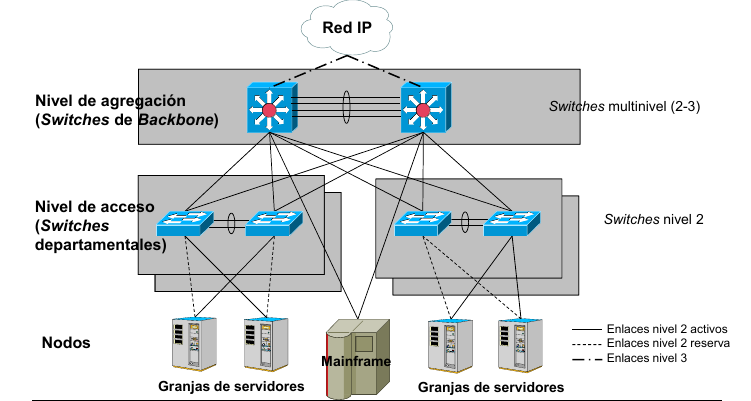
\includegraphics[width=\linewidth]{img/niveles.png}
\end{center}

La instalación de redundancias en el nivel 3 implica el uso de un protocolo de encadenamiento dinámico (OSPF, BGP), igual que en el caso de redes de área extendida (WAN).

A nivel 2, implica la aparición de bucles en los posibles caminos entre dos nodos de la red lo que lo hace incompatible con el protocolo \textit{Transparent Bridging} empleado en Ethernet. Este problema se resuelve con el \textit{Spanning Tree Protocol}, que se mejoró con el \textit{Rapid Spanning Tree Protocol}. Para optimizar el uso de VLANs se deben crear múltiples \textit{spanning trees}, solución proporcionada por \textit{Multiple Spanning Tree}.

En definitiva, si en la red de comunicación tenemos redundancias en un determinado nivel, es necesario emplear un protocolo que permita encontrar el mejor camino de un elemento a otro aún con las redundancias.

\subsection{Rapid Spanning Tree Protocol, RSTP}

Al aplicar este protocolo tenemos cada \textit{switch} asociado a un identificador que nos da su prioridad. El de mayor prioridad (menor identificador, ID1) se denomina \textit{switch} raíz. El siguiente en prioridad se le denomina \textit{switch} raíz alternativo (ID2).

Para cada puerto hay que determinar de que tipo es:
\begin{itemize}
\item Raíz. Da el mejor camino al \textit{switch} raíz

\item Designado. Proporciona a cada segmento de red conectado al \textit{switch} el mejor camino al \textit{switch} raíz. Es decir, que para algún nodo, su mejor camino hasta el nodo raíz implicar coger justo este enlace.

\item Alternativo. Otros.
\end{itemize}

Periódicamente, cada \textit{switch} genera una \textit{Bridge Protocol Data Unit, BDPU} y la envía a todos los \textit{switches} de la red.

\textcolor{red}{Mirar el ejemplo de moodle subido por la profesora. Explica bastante bien el protocolo}

\subsection{Detección de fallos en RSTP}
Puede producirse un fallo en un enlace conectado a un RP o DP, que se detecta directamente por los \textit{switches} que forman el enlace; o puede darse un fallo en un \textit{switch}. Si hay tres turnos seguidos en los que no se recibe BDPU de un \textit{switch}, se le da por muerto.

Tras el fallo, todos los \textit{switches} reconfiguran el \textit{spanning tree}, mediante intercambios locales de los \textit{switches} afectados por el cambio y el resultado se propaga al resto de la red.

\obs Hay otra versión de este mecanismo es el \textit{spanning tree normal}, en el que únicamente el \textit{root bridge} transmite BPDU. Sólo se detecta un problema tras 20 segundos (vida máxima) y tras esto recalculamos el \textit{spanning tree} completo.

\subsection{Redundancia en la conexión de servidores a nivel 2}
La redundancia básica en la conexión de un ordenador a una LAN se consigue mediante el uso de dos o más adaptadores de red.

Los puertos de estos adaptadores (un puerto por adaptador) tendrán la misma MAC, pero sólo uno de los adaptadores estará disponible. Si cae, el sistema activará otro. No afecta a los protocolos de niveles superiores.

\begin{defn}[EtherChannels]
Consiste en la agrupación de enlaces Ethernet donde todos los puertos poseen la misma MAC como si fuesen sólo 1 (y así lo ven desde arriba) y están activos simultáneamente.

Da mayor rapidez en la resolución de fallos y mejora el ancho de banda pero su implementación es costosa. Se requiere que ambos extremos de la conexión tengan soporte de \textbf{EtherChannels}. Los componentes de un \textbf{EtherChannel} no se pueden disgregar para conectar varios dispositivos distintos. A todos los efectos, es un único enlace.

\end{defn}

\subsection{Redundancia de las WAN}
Las redes WAN permiten establecer la interconexión entre elementos distantes de sistemas distribuidos. Se basan en el protocolo TCP/IP y se distinguen dos tipos de componentes: enlaces y unidades de encadenamiento (\textit{routers}).

La alta disponibilidad de las WAN se consigue teniendo muchos \textit{routers} y enlaces para que siempre haya caminos alternativos. La gestión del tráfico a través de las diferentes rutas se lleva a cabo con los protocolos de encadenamiento dinámico que estudiamos en Redes: OSPB y BGP.

\begin{defn}[OSPF]
Protocolo de encadenamiento dinámico eficaz y ampliamente utilizado en redes IP. Se basa en el conocimiento de toda la red y el empleo de Dijkstra para localizar el camino más corto. Se organiza la red en áreas dentro de las cuales los \textit{routers} encaminan los paquetes. Para cambiar de área se emplean los Area Border Gateways (\textit{routers} fronterizos)

El mensaje OSPF Hello se emplea para conocer la topología de la red con lo que cada \textit{router} conoce a sus vecinos. Y con el mensaje Link State se informa del estado de los enlaces.
\end{defn}

Se puede producir un fallo en OSPF por la caída de un enlace, que se detecta de forma inmediata, por la caída de un \textit{router}, que se detecta gracias al protocolo OSPF Hello, que sirve de \textit{keep-alive}. El mensaje Hello se intercambia cada 10 segundos. Si tras cuatro rondas no se han recibido Hello's de un \textit{router}, se le da por muerto.

Si en un caso concreto se requiere una configuración estática (estaciones de trabajo, por ejemplo) el \textit{router} por defecto que se asigna a estos dispositivos se convierte en un SPOF (Single Point Of Failure). Para evitarlo se emplea un cluster de \textit{routers} controlado con el protocolo \textit{Virtual Router Redundancy Protocolo, VRRP}

\begin{defn}[VRRP]
Protocolo de \textit{clustering} para \textit{routers} empleado para proporcionar redundancia en \textit{routers} en los casos en que representan un punto único de fallo en rutas de la red. El \textit{router} se sustituye por un \textit{virtual \textit{router}} formado por un \textit{router} activo y otro en \textit{stand-by}.

El \textit{router} de mayor prioridad será el activo y asume como propias una dirección IP y una MAC que habrán sido asignadas al \textit{router} virtual. Si cae el \textit{router} se activa otro.
\end{defn}

El \textit{router} activo envía mensajes Hello en \textit{multicast} cada x segundos. Si transcurre un tiempo predefinido sin recibir mensajes Hello, se da al \textit{router} por muerto y se activa el siguiente en prioridad. Este tiempo de espera predefinido es menor cuanto menor sea la prioridad. Así cuando esté un \textit{router} activo que no sea el inicial, tendrá más probabilidades de que se le dé por muerto, por lo que el \textit{router} principal tendrá más probabilidades de volver.

En el \textbf{fail-back} hay dos opciones:
\begin{itemize}
\item Si la configuración activa preempt, el \textit{router} de mayor prioridad asume el tráfico. Supone una breve interrupción del servicio mientras se produce el cambio.
\item Si la configuración desactiva preempt, se deja el \textit{router} actual como activo hasta un posible fallo, quedando el reincorporado como \textit{router} de backup.
\end{itemize}

\begin{defn}[Balanceador de carga]\label{cluster:LB}
Un balanceador de carga es un dispositivo capaz de distribuir peticiones entre un grupo de servidores para su proceso. Tiene como objeto aumentar la capacidad de proceso y la disponibilidad del servicio.

Previamente se realizaba este proceso en redes IP a través del DNS, resolviendo el mismo nombre por distintas IP pero esto no garantizaba que el servidor estuviera activo y los cambios del DNS son lentos al propagarse por la red.

Frente a un \textit{switch} que sólo maneja información de nivel 2 y un \textit{router} que sólo maneja información a nivel 3, el \textbf{Load Balancer, LB} también utiliza información de los niveles de transporte y aplicación para realizar el encadenamiento. Como mínimo debe garantizar que en TCP todos los paquetes de la misma conexión van al mismo servidor.
\end{defn}

Para emplear un LB, se asigna una dirección IP virtual (VIP), puerto y protocolo para el servicio a prestar; se asocian al LB los servidores que prestan el servicio y se definen unos mecanismos de distribución de carga y entrega de paquetes.

Cuando llega una petición, el LB decide qué servidor debe atenderla y se la reenvía. El servidor procesará la petición y devolverá una respuesta que será reenviada al cliente. Este último paso, según la configuración de entrega de paquetes, puede eliminarse siendo el servidor quien directamente responde al cliente. (\textit{Direct Server Return} vs \textit{Destination NAT})

El mecanismo de distribución de carga puede ser cualquiera: \textit{Round Robin}, alterno, menor número de conexiones, ponderado, mejor tiempo de respuesta, por origen de la petición, etc.

En cualquier caso es necesario considerar condiciones límite para realizar la entrega:
\begin{itemize}
\item Máximo número de conexiones permitido
\item Umbral de tiempo de respuesta
\item \textbf{Gracefull Shutdown}. No mandar más mensajes a un servidor que quiere desconectarse
\item \textbf{Tiempo de gracia}. Tiempo que se deja a un servidor desde que está activo hasta que se le envía tráfico, para permitir su estabilización adecuada.
\end{itemize}

Si todos los paquetes de respuestas pasaban por el LB, se puede detectar un fallo si un servidor deja de responder, se puede monitorizar en \textit{handshake} de TCP o los códigos de retorno de HTTP. Si no es así, se emplean pruebas de nivel 3 con ICMP echo/replay; a nivel 4, con apertura/cierre de conexiones TCP; o pruebas de nivel 7, tratar de conectar con la aplicación. Estos acciones las realizaría el LB para comprobar que el servidor esté activo.

El LB debe ser capaz de hacer que un cliente se conecte siempre a un mismo servidor para que se mantenga la sesión, que no está implementada de modo estándar en TCP/IP. Existen diferentes formas de hacerlo:
\begin{itemize}
\item Aplicando un algoritmo de balanceo por origen. Tiene el problema de que si varios clientes están tras una NAT son indistinguibles en este sentido.
\item Por concurrencia de conexiones. Una nueva petición de un cliente se envía al mismo servidor que mantiene la actual
\item Cookies o identificadores SSL que guarden información de la sesión. Requiere analizar el paquete e impide que el balanceo se haga por paquete. Es necesario partir la conexión TCP en el LB
\end{itemize}

\subsection{Redundancia en los sistemas de almacenamiento de la información}
La información es el punto más crítico de todo sistema informático puesto que perder datos o no tenerlos disponibles adecuadamente puede ser fatal para cualquier tipo de negocio.

La redundancia de este tipo de elementos es más compleja pues es necesario mantener la consistencia y garantizar que los elementos de procesamiento redundantes accedan a la misma copia de la información.

Existen diferentes arquitecturas de almacenamiento. Veamos algunas:
\begin{itemize}
\item \textbf{Conexión directa (Direct Attached Storage, DAS)}. Consiste en conectar el dispositivo de almacenamiento directamente al servidor o estación de trabajo, es decir, físicamente conectado al dispositivo que hace uso de él. Normalmente se usa directamente el protocolo SCSI en alguna de sus variantes.

\item \textbf{Conexión a red (Network Attached Storage, NAS)}. Es el nombre dado a una tecnología de almacenamiento dedicada a compartir la capacidad de almacenamiento de un computador (Servidor) con computadoras personales o servidores clientes a través de una red (normalmente TCP/IP), haciendo uso de un Sistema Operativo optimizado para dar acceso con los protocolos CIFS, NFS, FTP o TFTP.

\item \textbf{Red de área de almacenamiento (Storage Area Network, SAN)}. Red dedicada al almacenamiento que está conectada a las redes de comunicación de una compañía. Además de contar con interfaces de red tradicionales, los equipos con acceso a la SAN tienen una interfaz de red específica que se conecta a la SAN. Utiliza fibra óptica como medio de transporte y el protocolo \textit{FibreChannel}

\item \textbf{Internet SCSI (iSCSI)} Estándar que permite el uso del protocolo SCSI sobre redes TCP/IP

\item \textbf{FibreChannel Over IP (FCIP)} Encapsula el protocolo FibreChannel sobre IP estableciendo túneles FC sobre TCP.

\item \textbf{Internet Fibre Channel Protocol (iFCP)} Implementa FC sobre IP pero no en modo túnel sino interpretando el protocolo FC.
\end{itemize}

Uno de los métodos para mantener redundante la información en unos ciertos discos es el uso de \textbf{Redundan Array of Independen Disks, RAID}, que ya hemos estudiado en otras asignaturas.

\begin{center}
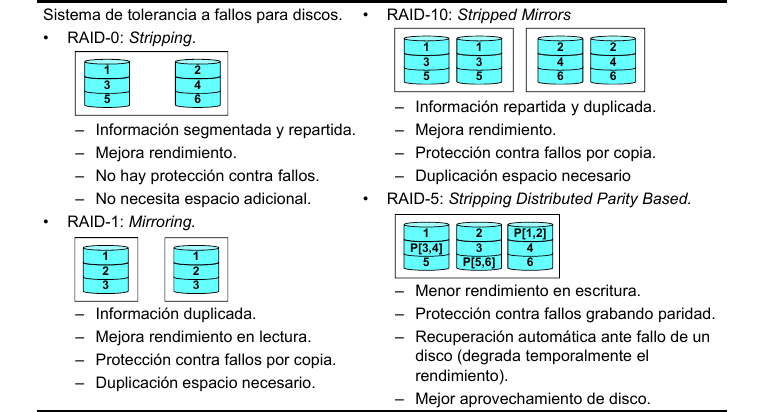
\includegraphics[width=\linewidth]{img/raid.png}
\end{center}

Los servidores de disco proporcionan herramientas autónomas para garantizar la copia de la información, y garantizar así su disponibilidad para los servidores que la utilizan, liberando así a los servidores de aplicaciones de la tarea de realización de las copias.

Estas copias pueden ser locales o remotas. Estas últimas podrían ser síncronas o asíncronas.

Dentro de las copias locales existen dos tipos: clonación de discos (se copia la información de una Unidad Lógica\footnote{Viene a ser como las particiones lógicas pero que afectan a diferentes discos, no sólo a 1} a otra) y las copias instantáneas (\textit{Snapshots o Flash Copy}).

\begin{defn}[Flash Copy]
Copia de una Unidad Lógica en el instante que se solicita, copiando los punteros a los sectores que contienen la información.

En caso de que haya una actualización de un sector, se copia la información antigua y se actualiza el puntero de la copia instantánea.

Se emplean para generar una copia consistente de la información en un momento preciso para su uso posterior.

\obs Básicamente guardas un puntero a la posición guardada. Si no la modifican, pues ya lo tienes. Si se modifica esa parte del disco, mueves la antigua información a otro sitio y actualizas tu puntero.
\end{defn}

Las copias remotas \textbf{síncronas} consisten en que la actualización de la información del servidor primario se copia a los secundarios y el proceso no finaliza hasta que no se ha actualizado la información en todos los servidores, lo que da lugar a una alta latencia de escritura. \textbf{Empleado para realizar copias locales que garanticen la alta disponibilidad}

En las \textbf{asíncronas}, una vez se actualiza el primario se guardan los cambios en un buffer y se van aplicando en el resto de servidores mediante un proceso en paralelo. Requiere un protocolo de sincronización. \textbf{Empleado para realizar copias remotas que permitan la recuperación ante desastres} \href{http://searchdatacenter.techtarget.com/es/consejo/Ventajas-e-inconvenientes-de-la-replicacion-remota-en-la-recuperacion-de-desastres}{Leer más}

Las posibles averías en discos físicos individuales son resueltas por la arquitectura RAID. Si se producen averías en una Unidad Lógica (LUN) completa o en un servidor de disco se siguen los siguientes pasos:
\begin{enumerate}
\item[1] \textbf{Fail-Over}. Se interrumpe la copia remota y la LUN secundaria pasa a principal. Para ello se notifica al servidor de proceso que debe usar a LUN secundaria y se comienza a registrar los cambios.

\item[2] \textbf{Fail-Back} Se copia el secundario activo al primario una vez recuperado. Para ello se detiene el trabajo del servidor de proceso, se restablece la copia y se notifica al servidor de proceso que puede seguir utilizando el primario.
\end{enumerate}


\subsection{Redundancia en los sistemas de proceso}
Este tipo de redundancia se consigue mediante la asociación de los elementos de proceso (servidores) en grupos (clusters) que realizan una tarea común.

Cada servidor ejecutará un determinado número de grupos de servicio compuesto por una identidad de red (direcciones a las que el servicio responde), un conjunto de información almacenada en discos físicos o LUNs y un conjunto de procesos.

Si un servidor de un cluster falla, los grupos de servicio que soporta deben ser trasladados a otro elemento del cluster.

Básicamente un grupo de servicios es un conjunto de actividades que desempeña un servidor, es decir, procesos que ejecuta, direcciones a las que responde y memoria que usa. Si el servidor cae y no puede desempeñar estas actividades, otro tiene que ocupar su lugar.

Hay tres tipos de clusters según su modo de funcionamiento y gestión.
\begin{enumerate}
\item[1] \textbf{Clusters Activo-Pasivo o asimétricos:} Cada grupo de servicio se ejecuta en un nodo. Existen nodos de reserva en stand-by para ejecutarlos en caso de fallo.

\begin{defn}[Heartbeat]
``In computer clusters, heartbeat network is a private network which is shared only by the cluster nodes, and is not accessible from outside the cluster. It is used by cluster nodes in order to monitor each node's status and communicate with each other.'' -{}- Wikipedia.\footnote{\url{http://en.wikipedia.org/wiki/Heartbeat_network}}\\

Es uno de los puntos críticos de un \textit{cluster} de alta disponibilidad. Si falla se producirá la activación simultánea de ambos nodos, generando conflictos y caída del servicio.

Puede implementarse como una red de área local o mediante la escritura en una sección reservada de disco compartido.
\end{defn}

Para aumentar la fiabilidad del \textbf{heartbeat} se pueden tomar diversas medidas:
\begin{itemize}
\item Eliminar SPOF en los mecanismos de transporte del heartbeat.
\item Emplear dos heartbeat (dos redes o red+disco). Actuar sólo en caso de fallo
de ambos.
\item Emplear redes independientes lo más simples posibles: cable cruzado para
dos nodos, o segmentos de LAN con \textit{switches} independientes.
\item Vigilar el correcto funcionamiento de los procesos que generan y atienden los
hearbeats en cada nodo. Instalar un watchdog local que los rearranque en caso de caída.
\end{itemize}

Existe una serie de \textbf{problemas a la hora de rearrancar en el servidor secundario} en el caso de fallo de uno de los nodos.

Si el cambio en la dirección IP se realiza sobre un adaptador con otra dirección MAC, la caché ARP de los clientes mantendrá la antigua hasta que detecten la nueva situación. Por ello se asume también la antigua dirección MAC.

Cuando la parada es no planificada (se dio un fallo en el sistema) se perderán datos de las aplicaciones, las cachés de disco y/o transacciones que se estuvieran realizando. Es por ello que el arranque de servicios en el servidor de reserva se hace siguiente los procedimientos de arranque tras un cierre anormal:
\begin{itemize}
\item Revisión de la consistencia de los sistemas de archivos a nivel de sistema operativo.
\item Revisión de la consistencia de los datos en disco a nivel de aplicación (por ejemplo, bases de datos).
\item Rollback de las transacciones activas en el momento del fallo.
\end{itemize}

En caso del fail-back este proceso será planificado, realizándose un cierre ordenado. En ambos casos se interrumpirá el servicio.

\item[2] \textbf{Clusters Activo-Pasivo cruzados o simétricos:} Cada grupo de servicio se ejecuta en un nodo. Todos los nodos ejecutan grupos de servicio. En caso de fallo de un nodo, el resto se hacen cargo de la ejecución de sus grupos de servicio.

El modelo es similar al anterior, pero con grupos de servicios activos en ambos nodos. Cada nodo tiene direcciones de servicio fijas y, en caso de fallo, el resto de nodos deberá hacerse cargo de todas las direcciones.

En este modelo nunca se parará el sistema y, si no hay fallo, hay menos capacidad de proceso desaprovechada.

Por otro lado, este modelo tiende a sobrecargar los nodos y, debido a la carga de trabajo de los supervivientes tras un fallo, es posible que les cueste absorber la carga del nodo caído. Además, es imposible asignar dos o más direcciones MAC en el adaptador de un nodo de modo que los clientes del nodo caído deberán realizar un nuevo ARP para conectar con otro nodo.


\item[3] \textbf{Clusters Activo-Activo:} Cada grupo de servicio se ejecuta en múltiples nodos. El fallo de uno de los nodos no supone la caída del grupo de servicio.

En este modelo existe un mecanismo de balanceo de carga para asignar las peticiones de los clientes a alguno de los nodos activos, que realiza el reparto de la carga y la verificación de la actividad.

Si falla uno nodo no cae el grupo de servicio e incluso, dependiendo del tipo de aplicación, las conexiones activas en el momento del fallo pueden mantenerse también.

El cluster debe incluir soluciones para el acceso compartido a discos en lectura y escritura, creación de áreas de memoria compartida entre los nodos del cluster, consistencia de la información distribuida entre los distintos nodos, etc.

\begin{example}
Ya vimos en el tema 2 la arquitectura de un servidor de aplicaciones J2EE, que es la que muestra la siguiente imagen:
\begin{center}
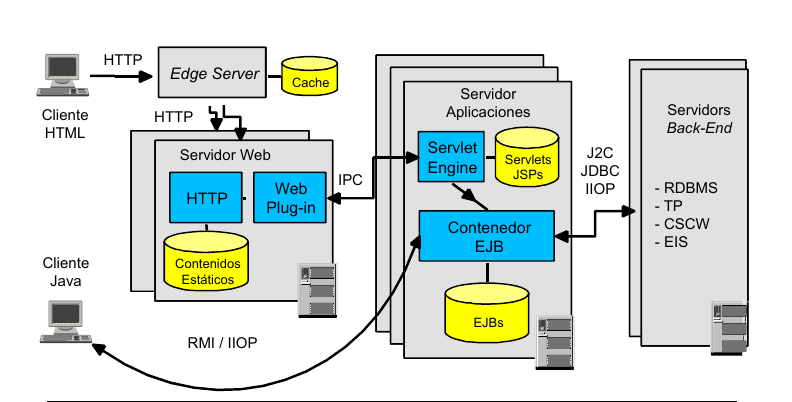
\includegraphics[width=\linewidth]{img/j2ee.png}
\end{center}

Se trata de un \textbf{cluster Activo-Activo}.

El balanceo de carga entre servidores Web lo realiza el Edge Server y el balanceo de carga entre Servlet Engines lo realiza el Web Plug In.

La alta disponibilidad en el acceso a los contenedores EJB y a los servicios de Back End es proporcionada por IIOP (corba) y por mecanismos de \textit{clustering} respectivamente.

La continuidad de la sesión entre distintas Servlet Engines se obtiene mediante el mantenimiento común de los datos de sesión. Este soporte común se puede conseguirse mediante una tabla de sesiones en una BD compartida, un gestor de réplica centralizado (Redundado para evitar SPOF) o un gestor de réplica distribuido.
\end{example}

\end{enumerate}

\section{Recuperación ante desastres}

Un desastre es cualquier circunstancia que puede producir un fallo en la operativa del negocio de una empresa. Pueden ser naturales, humanos, accidentes ...

Aunque tengan poca probabilidad, el impacto puede ser muy alto (por ejemplo, si se queman tus servidores de datos). Para garantizar la recuperación ante un desastre no basta con las técnicas de alta disponibilidad vistas hasta ahora sino que son necesarias nuevas técnicas que se presentan en esta sección.

Veamos algunas definiciones necesarias para entender los conceptos que analizaremos en este apartado:

\begin{defn}[Recovery\IS Point Objective (RPO)][Recovery\IS Point Objective]\index{RPO}
Instante de tiempo al que se es capaz de recuperar la información existente en el sistema tras un fallo. Si no es 0, habrá perdida de datos
\end{defn}

\begin{defn}[Recovery\IS Time Objective (RTO)][Recovery\IS Time Objective]\index{RTO}
Tiempo que se tarda en recuperar los sistemas tras producirse un fallo. Si no es 0, habrá interrupciones de servicio.
\end{defn}

Menores valores de RTO y RPO requieren mayor coste por lo que hay que analizar bien las necesidades del servicio.

Hay unas reglas básicas en el diseño de arquitecturas tolerantes a desastres:
\begin{enumerate}
\item Proteger datos y nodos de proceso mediante distribución geográfica.

Cuanto más alejados se encuentren, mayor seguridad, pero mayor
complejidad y coste.

\item Proporcionar a los CPDs redundancia en el suministro de energía.
Preferiblemente con acometidas independientes, a través de rutas alternativas de
distribución y proporcionadas por distintas entidades suministradoras.

\item Proporcionar a los CPDs redundancia en el acceso de telecomunicaciones. Con
las mismas consideraciones que en el caso anterior.

\item Generar copias consistentes de la información, garantizando la capacidad de
recuperar los datos desde ellas.
\begin{itemize}
\item \textbf{Copias off-line:} backups en cinta. Proporcionan un RPO elevado.

Puesto que hay que hacerlos de forma consistente, debe detenerse las aplicaciones mientras se realiza el backup o emplear técnicas de copia instantánea.

Además debe probarse que la información se restaura correctamente.

\item \textbf{Copias on-line:} réplicas directas de disco a disco. Proporcionan un RPO reducido.

Los mecanismos más habituales, ordenados de menor a mayor fiabilidad son:
\begin{enumerate}
\item Scripts de usuario. Automatizados por planificador.
\item Réplicas basadas en software en los sistemas de proceso, a distintos niveles:

\item Réplicas basadas en nivel de driver: mirroring remoto.
\item Réplicas basadas en el hardware de los servidores de disco: síncronas y
asíncronas, estudiadas previamente.
\end{enumerate}
\end{itemize}

\end{enumerate}

\subsection{Arquitecturas de CPDs orientadas a la recuperación ante desastres}\label{cluster:disaster}
\textbf{Clusters a nivel de campus}
\begin{itemize}
\item Los elementos del cluster se distribuyen entre dos edificios próximos.
\item Extensión de LAN y SAN entre ambos edificios, normalmente con cableado propio.
\item Es posible la copia síncrona de información entre servidores de disco.
\item El funcionamiento lógico es como un cluster local: Proporciona alta disponibilidad.
\item Protege frente a desastres que ocurran en un único edificio.

\end{itemize}

\textbf{Clusters metropolitanos}
\begin{itemize}
\item Similar al anterior, pero con edificios en ubicaciones distantes que no excedan el rango en el que es posible realizar copia síncrona de la información.
\item Extensión de LAN y SAN con enlaces alquilados de alta velocidad (``fibra oscura'', WDM).
\item Protege frente a desastres locales.

\end{itemize}

\textbf{Clusters continentales}
\begin{itemize}
\item Sin límite de distancia entre centros.
\item Requieren conexión a través de red WAN.
\item Protege frente a desastres en áreas extensas (región o estado), según la distancia entre centros.

\end{itemize}
\newpage
\textbf{Soluciones mixtas}
\begin{itemize}
\item Cluster local o metropolitano para garantizar alta disponibilidad, añadiendo un cluster continental para garantizar recuperación ante desastres.

\end{itemize}

\begin{center}
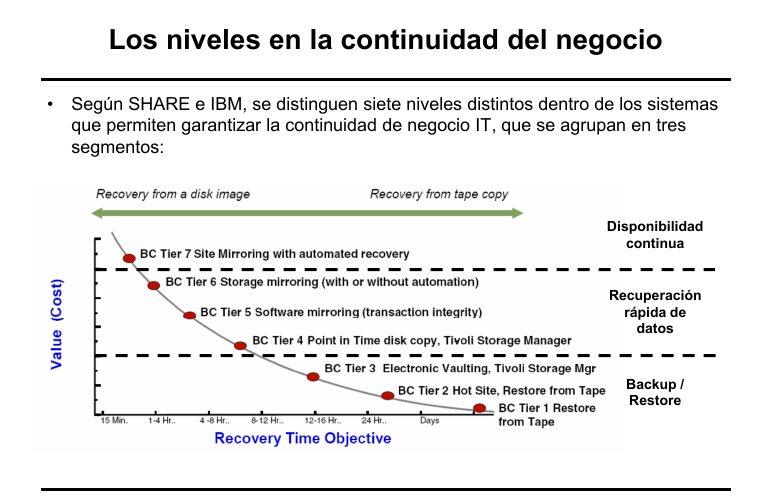
\includegraphics[width=\linewidth]{img/continuidad_negocio.png}
\end{center}

\subsection{Resumen de tipos de clusters}
En resumen, en este tema se han visto 4 tipos de clusters:
\begin{itemize}
	\item \textbf{High performance cluster} : \ref{cluster:HP}
	\item \textbf{Load balancer} : \ref{cluster:LB}
	\item \textbf{Cluster orientado a la recuperación ante desastres} : \ref{cluster:disaster}
	\item \textbf{Cluster tolerante a fallos} : \ref{cluster:FT}
\end{itemize}
